\documentclass[article,a4paper,oneside,10pt]{memoir}

% -------------------------------------------------------------------------- %
% Page Layout                                                                %
% -------------------------------------------------------------------------- %
\setlrmarginsandblock{0.142857111\paperwidth}{0.142857111\paperwidth}{*}
\setulmarginsandblock{0.111111111\paperheight}{*}{1.25}
\checkandfixthelayout
\newfixedcaption{\figcaption}{figure}
\newfixedcaption{\tabcaption}{table}
\captiontitlefont{\small}
\captionnamefont{\bfseries\small}
\captiondelim{: }

% -------------------------------------------------------------------------- %
% Bibliography                                                               %
% -------------------------------------------------------------------------- %
\renewcommand{\bibsection}{%
    \chapter{References}%
    \prebibhook}
\bibintoc
\renewcommand{\cftdot}{\textcolor{gray}{.}}
\renewcommand{\cftchapterdotsep}{\cftdotsep} % Chapters have dots in ToC
\renewcommand{\cftsectiondotsep}{\cftnodots} % Sections have no dots in ToC


% -------------------------------------------------------------------------- %
% Chapter and Section Headings                                               %
% -------------------------------------------------------------------------- %
\makeatletter
\makechapterstyle{alpensec}{%
  \chapterstyle{default}
  \setlength{\beforechapskip}{3.5ex \@plus 1ex \@minus .2ex}
  \renewcommand*{\chapterheadstart}{\vspace{\beforechapskip}}
  \setlength{\afterchapskip}{2.3ex \@plus .2ex}
  \renewcommand{\printchaptername}{}
  \renewcommand{\chapternamenum}{}
  \renewcommand{\chaptitlefont}{\sffamily\LARGE\bfseries}
  \renewcommand{\chapnumfont}{\chaptitlefont}
  \renewcommand{\printchapternum}{\chapnumfont \thechapter\quad}
  \renewcommand{\afterchapternum}{}}

\renewcommand{\section}{%
  \sechook%
  \@startsection{section}{1}%  level 1
      {\secindent}%            heading indent
      {\beforesecskip}%        skip before the heading
      {\aftersecskip}%         skip after the heading
      {\sffamily\secheadstyle}} % font

\makeatother

\chapterstyle{alpensec}


% -------------------------------------------------------------------------- %
% Packages                                                                   %
% -------------------------------------------------------------------------- %
\usepackage[%
        bookmarksnumbered=true,
        colorlinks=true,
        linkcolor=cyan!50!blue,
        citecolor=violet,
        urlcolor=purple,
    ]{hyperref}
\usepackage[light,nott]{kpfonts}
\usepackage{microtype}
\usepackage[english]{babel}
\usepackage[T1]{fontenc}
\usepackage[utf8]{inputenc}
\usepackage{xcolor-solarized}
\usepackage{lipsum}
\usepackage{graphicx}
% -------------------------------------------------------- %
% Minted defines the listing  environment via the newfloat %
% package. This leads to  the listoflistings being typeset %
% on the  section level,  with the entries  being indented %
% too far.  We therefore create our own listings float and %
% corresponding listof before loading minted.              %
%                                                          %
% See:                                                     %
% memman.pdf page 170                                      %
% https://github.com/gpoore/minted/issues/67               %
% -------------------------------------------------------- %
\newcommand{\listingname}{Listing}
\newcommand{\listlistingname}{List of Listings}
\newlistof{listoflistings}{lol}{\listlistingname}
\newfloat{listing}{lol}{\listingname}
\newlistentry{listing}{lol}{0}
\usepackage{minted}
\usepackage{tcolorbox}
\renewcommand{\listingscaption}{\small\bfseries Listing}


% -------------------------------------------------------------------------- %
% Macros and Config                                                          %
% -------------------------------------------------------------------------- %
\newcommand\code[1]{\texttt{#1}}

\DeclareTextFontCommand{\emphc}{\color{solarized-red}\em}

\tcbuselibrary{minted}
\tcbset{
    listing and text,
    listing engine=minted,
    %title=\textsf{\bfseries Code \hfill \LaTeX{} Output},
    minted language=text,
    minted options={autogobble}}

% -------------------------------------------------------------------------- %
% Title                                                                      %
% -------------------------------------------------------------------------- %
\title{\textsf{\Huge  The Black Magic of Floats in \LaTeX}}
\author{Raphael Frey\\[2mm]\small%
    \href{https://github.com/alpenwasser/TeX/tree/master/floats}
         {\nolinkurl{https://github.com/alpenwasser/TeX/}}}

\date{\vspace{1em}\today}

% ************************************************************************** %
\begin{document}
% ************************************************************************** %


\maketitle

\begin{abstract}
    The behavior  of floats can  often be  confusing for the  uninitiated, and
    yield  unexpected results. This  document gives  a brief  overview on  the
    subject, primarily based on Leslie  Lamport's \emph{\LaTeX{} -- A Document
    Preparation System} \cite{lamport}.

    I will not cover every possible edge case, but present some usage examples
    and common problem one tends to run into while working with floats.
\end{abstract}

\tableofcontents*
\listoflistings*
\listoffigures*
\listoftables*


% ========================================================================== %
\newpage
\chapter{What Are Floats, Anyway?}
\label{chap:what-are-floats}
% ========================================================================== %

Normal text  is broken  by \TeX{} across  lines and  pages automatically. Some
content, such as images, are not  well-suited to being split into pieces. That
is what floating environments are for: To provide a way to put such content in
a place where it does not need to be broken; a way for it to \emph{float} to a
suitable location for an optimal overall result.

Two  such  floating environments  are  provided  by \LaTeX{}  by  default: The
\verb|figure|   and  the   \verb|table|\footnotemark  environment. There   are
packages   which  define   more  floating   environments  (for   example,  the
\verb|listings| packages can  let its code listings float, if  so desired), or
the user may define their own floating environments, if they so wish.

\footnotetext{%
    Because confusion is fun: The \texttt{table} environment does not actually
    typeset  a table.   That is  what \texttt{tabular},  \texttt{tabularx} and
    similar environments are for. See  \cite{mori:tables} for an overview. The
    \texttt{table}  environment is  merely a  floating container  intended for
    containing tabular content.}

Fundamentally, the only important difference between these environments is how
they  are  captioned  and  numbered: \verb|figure|  environments  will  get  a
different caption and  number to a \verb|table|  environment. However, one may
in principle put pretty much  anything one desires into either environment. As
long  as  the  code  itself  is  valid,  \LaTeX{}  will  not  complain. Figure
\ref{fig:lipsum} and Table \ref{lipsum} demonstrate this by placing some Lorem
Ipsum text inside their environments.

The floating behavior can be demonstrated by the fact that, in the source code
of this  document, Figure \ref{fig:lipsum} and  Table \ref{tab:experiment} are
placed almost right  after this sentence. In the resulting  document, they may
be placed  wherever \LaTeX{}  deems most  suitable\footnotemark.

\footnotetext{%
    \LaTeX{} usually tries  to place floats either  at the top of  a page, the
    bottom of a page, or on a separate page. See \ref{chap:placement} for more
    information.}


\begin{figure}
    {\color{gray}\centering\small\lipsum[2]}
    \caption{A \texttt{figure} environment with placeholder text}
    \label{fig:lipsum}
\end{figure}

\begin{table}
    \centering
    \caption{Results for an experiment}
    \label{tab:experiment}
    \begin{tabular}{ll}
        \toprule
        \scshape Experiment Input & \scshape Experiment Output \\
        \midrule
        interesting thing         & interesting result!        \\
        boring thing              & mildly surprising result   \\
        weird thing               & very unexpected result     \\
        fascinating thing         & machine broke              \\
        Xenomorph XX121           & dead scientists            \\
        \bottomrule
    \end{tabular}
\end{table}


Because  captions are  a moving  argument (Section  3.5.1 in  \cite{lamport}),
fragile  commands  such  as  linebreaks   inside  them  must  be  preceded  by
\verb|\protect|, as shown  in the caption of Figure  \ref{fig:protect} and the
code in Listing \ref{lst:figure}.

\begin{figure}
    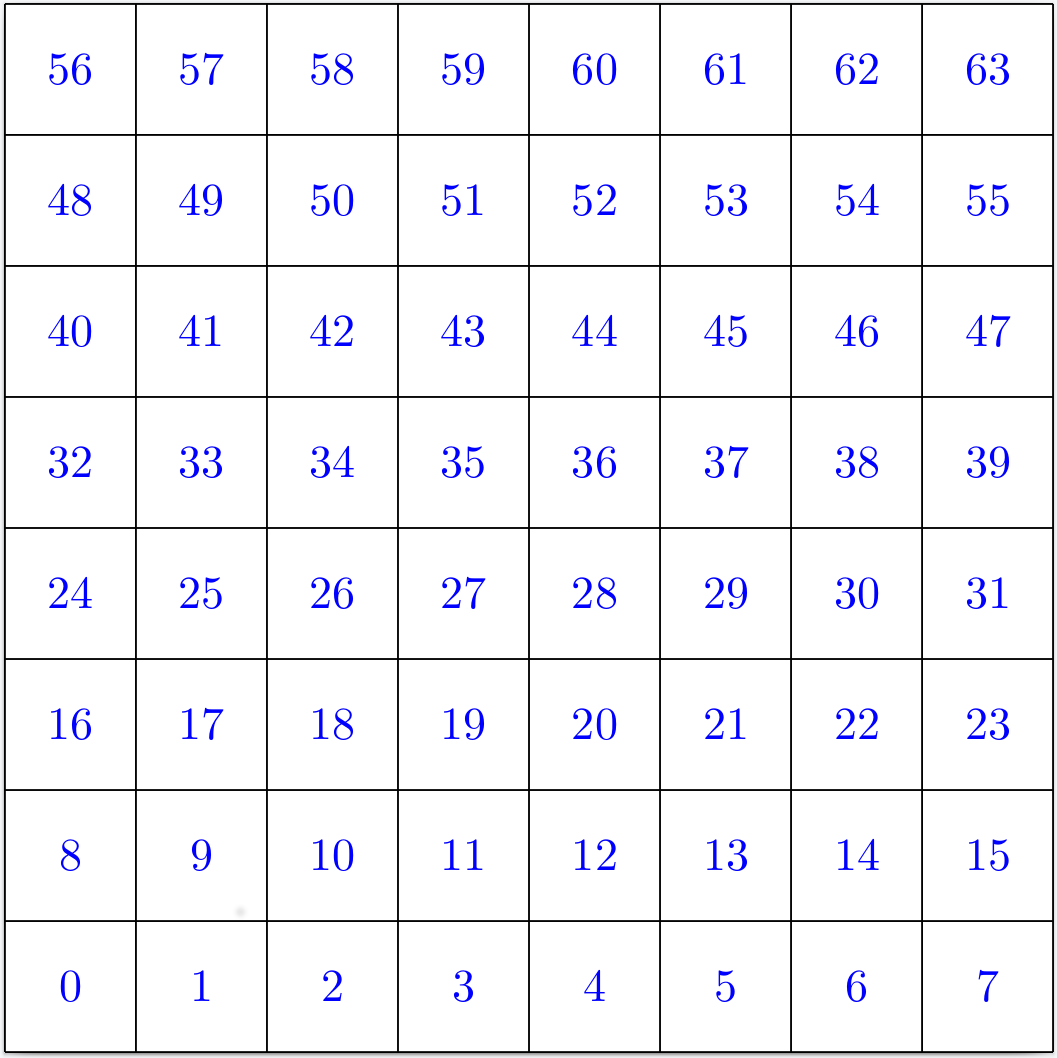
\includegraphics[height=3cm,width=4.5cm]{images/grid8cm.png}
    \caption[Linebreaks in Captions]{%
        One can  place arbitrary  content inside a  \code{figure} environment,
        though this does not usually make much sense.\protect\\
        Note  that  you can  also  have  linebreaks inside  a  \code{caption},
        like   here,  but   it  requires   the  \code{\textbackslash{}protect}
        command,   and   there    must   be   no   empty    line   after   the
        \code{\textbackslash\textbackslash}. See Listing  \ref{lst:figure} for
        the code.}
    \label{fig:protect}
\end{figure}

The \verb|\caption| command can only be  used inside a floating environment by
default.   If  you require  captions  for  non-floating arguments,  there  are
packages which provide such facilities,  as well as more caption customisation
options,   see   \cite{ctan:package:caption,ctan:topic:caption}  and   Chapter
\ref{chap:alternatives} of this document.


% ========================================================================== %
\chapter{Basic Usage}
\label{chap:basic-usage}
% ========================================================================== %

Listing \ref{lst:figure}\footnotemark  shows the  basic code for  including an
external  graphics file  inside a  \verb|figure| environment  and providing  a
caption to go along with it.

\footnotetext{%
    Incidentally, Listing \ref{lst:figure}  is one of those cases  where a new
    type  of floating  environment  has been  provided; in  this  case by  the
    \texttt{minted} package.}

\begin{listing}
    \begin{tcblisting}{%
            title={\bfseries\sffamily Figure Environment with External Picture},
            minted language=tex,
            listing only,
            minted options={autogobble,escapeinside=||}}
        \begin{figure}
            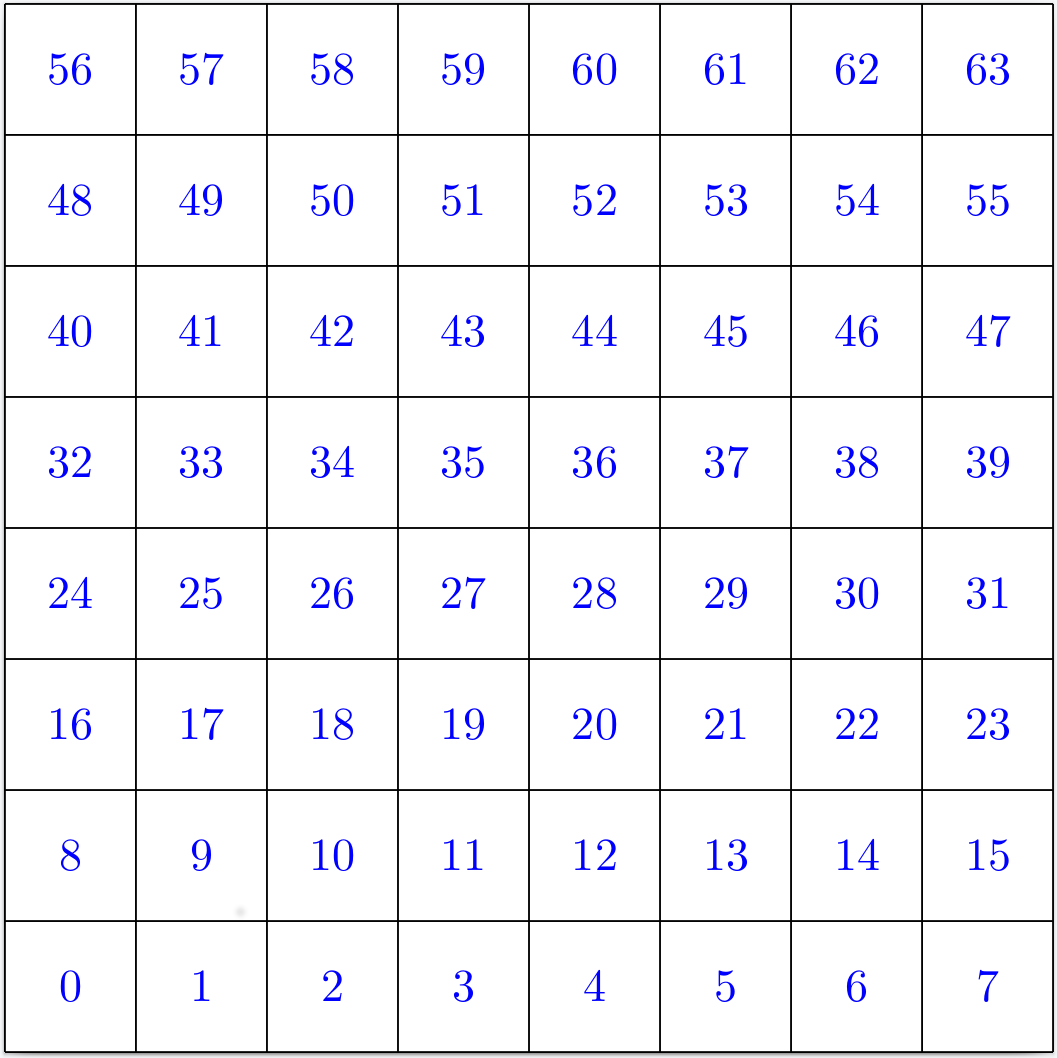
\includegraphics[height=3cm,width=4.5cm]{images/grid8cm.png}
            \caption{%
                One can  place arbitrary content inside  a figure environment,
                though this does not usually make much sense.|\textcolor{solarized-red}{\bfseries\textbackslash{}protect\textbackslash\textbackslash}|
                Note  that you  can  also have  linebreaks  inside a  caption,
                like  here,   but  it  requires   the  \textbackslash{}protect
                command,  and   there  must  be   no  empty  line   after  the
                \textbackslash\textbackslash. See Listing \ref{lst:figure} for
                the code.}
            \label{fig:distorted-grid}
        \end{figure}
    \end{tcblisting}
    \caption{%
        Code block for including a graphics in a figure and including a forced
        linebreak in a caption with a \code{\textbackslash{}protect} command}
    \label{lst:figure}
\end{listing}


It is  often desirable to center  a table or a  picture, in which case  we add
a  \verb|\centering|  directive  into  the environment,  as  done  in  Listing
\ref{lst:centering}\footnotemark.

\footnotetext{%
    There     exists     also    a     \texttt{\textbackslash{}begin\{center\}
    \ldots   \textbackslash{}end\{center\}}   environment. For  the   curious,
    some    information    on    the     differences    between    that    and
    \texttt{\textbackslash{}centering} can be found at
    \cite{stackexch:center-centering,texblog:center-centering}}

\begin{listing}
    % ---------------------------------------------------- %
    % Note that  we have to  do a bit of  workaround magic %
    % inside the  escaped part  of the  minted environment %
    % because it drops us back into LaTeX.                 %
    % ---------------------------------------------------- %
    \begin{tcblisting}{%
        title={\bfseries\sffamily Tabular Inside Table, Centered},
        listing only,
        minted options={autogobble,escapeinside=||}}
        \begin{table}
            |\textcolor{solarized-red}{\textbf{\textbackslash{}centering}}|
            \caption{Results for an experiment}
            \label{tab:experiment}
            \begin{tabular}{ll}
                \toprule
                \scshape Experiment Input & \scshape Experiment Output \\
                \midrule
                interesting thing         & interesting result!        \\
                boring thing              & mildly surprising result   \\
                weird thing               & very unexpected result     \\
                fascinating thing         & machine broke              \\
                Xenomorph XX121           & dead scientists            \\
                \bottomrule
            \end{tabular}
        \end{table}
    \end{tcblisting}
    \caption[Centering a Float]{%
        Centering  a  \texttt{tabular}  environment  inside  a  \texttt{table}
        floating     environment. This    is     the     code    for     Table
        \ref{tab:experiment}.}
    \label{lst:centering}
\end{listing}


You may have noticed that the  \verb|\caption| is placed above the content for
tables  and below  the picture  in  a \verb|figure|  environment. This is  not
prescribed by  \LaTeX, obviously, and  will depend  on the style  guide you're
following or your own preferences. All I will  say on the subject is that most
tables I've seen  had their caption above  the table and most  images had them
below the picture.

\emphc{What does matter, however,  is where the \texttt{\textbackslash{}label}
is put!} In order  to pick up the  correct number, it must  always come either
inside the  \verb|\caption| command to which  is is supposed to  be connected,
or  after  it.   If  you  put  it  before  the  \verb|\caption|  command,  the
\verb|\label| will  pick up whichever counter  was the last active  one before
the \verb|\caption|, which can be anything  (another picture or table or float
of some sort, but also a chapter, section or similar). This is a mistake which
is easily made and often hard to detect.

Lastly, note  the optional argument  to the \verb|\caption| command. If  it is
given, it will be the text  for the entry in the \verb|listof...| command. See
Listing \ref{lst:caption-opt-arg}.

\begin{listing}
    \begin{tcblisting}{%
            title={\bfseries\sffamily%
                Optional Argument for \code{\textbackslash{}caption} Command},
            minted language=tex,
            listing only}
            \caption[This is the text for the List of <something> entry]{
                This is the  text which goes below/above the  float. It can be
                rather  long, depending  on how  much explanation  the content
                of  the  float requires  (remember:  because  a float  is  not
                necessarily right  where you  write about  its content  in the
                main  body of  text,  it might  be useful  for  the reader  to
                understand its  content without having  to go and  dig through
                the main text),  and in such cases, it does  not make sense to
                have the entire text of the caption in the List of entry.}
    \end{tcblisting}
    \caption{%
        Optional Arguments  to the \code{\textbackslash{}caption}  command for
        the \code{List of \ldots} entry.}
    \label{lst:caption-opt-arg}
\end{listing}


% ========================================================================== %
\clearpage
\chapter{Placement Options}
\label{chap:placement}
% ========================================================================== %

Placement  options  allow you  to  influence  \LaTeX's placement  behavior  of
floats, with more or less vehemence.

\emphc{Whatever your preferences, only use placement options once your text is
(almost) complete.} Otherwise you will end up needing to change them again and
again and again, causing a lot more work. Also, it is quite easily possible to
overlook  a  bad placement  option  from  an  earlier  version of  a  document
which  makes  you jump  through  hoops  trying to  get  the  best result  even
though  \LaTeX{} would  actually do  the  right thing  if you  would just  let
it\footnotemark.

\footnotetext{%
    I am  obviously \emph{not}  speaking from  personal experience  here. I am
    smarter than that, I assure you.}

\begin{listing}
    \begin{tcblisting}{%
            title={\bfseries\sffamily%
                Placement Options},
            minted language=tex,
            listing only,
            minted options={autogobble,escapeinside=||}}
            \begin{float type}[|\textcolor{solarized-red}{loc}|] body \end{float type}
    \end{tcblisting}
    \caption{Placement options for floats}
    \label{lst:placement-options}
\end{listing}

Listing \ref{lst:placement-options} contains the basic  syntax of a float with
placement options. The  \code{loc} argument can be  a sequence of one  to four
letters and  an exclamation mark. The meaning  of these options is  as follows
(paraphrased from \cite{lamport}):

\begin{itemize}
    \item  [\code{h}] \emph{Here:}  at  the  location in  the  text where  the
        environment is  in the  source code. Does  not work  for double-column
        floats in two-column documents.

    \item [\code{t}] \emph{Top:} at the top of a text page.

    \item [\code{b}]  \emph{Bottom:} at  the bottom of  a text  page. Does not
        work for double-column floats in two-column documents.

    \item [\code{p}] \emph{Page of floats:} on a separate page containing only
        floats, but no text.

    \item [\code{!}] \emph{Try harder:} tells  \LaTeX{} to try harder to place
        the float  at the earliest possible  place in the document  allowed by
        the  rest  of  the  argument. The  meaning  of  \emph{try  harder}  is
        elaborated in Section \ref{chap:innards}.

        This also  overrides a \verb|\suppressfloats| (see  below) command for
        the float to which it belongs.
\end{itemize}

The  default  value for  \code{loc},  if  it  is  not specified  manually,  is
\code{tpb}, meaning \LaTeX{} may put the float  at the top of a text page, the
bottom of a text page, or on a separate page containing only floats.

When  an  optional  \code{loc}  argument   is  given,  make  sure  to  specify
enough  options to  allow  \LaTeX{} sufficient  flexibility  with placing  the
floats. Otherwise a  float and all  subsequent floats  can end up  being saved
until the end of a chapter or  document, potentially causing \TeX{} to run out
of memory  or producing  a result which  does not make  sense from  a document
design point of view.


Additionally, there exists  the \verb|\supressfloats[loc]| command. This tells
\LaTeX{} not to put any additional  floats on the current page. \code{loc} can
be:

\begin{itemize}
    \item [\code{t}] No more figures at the top of the current page.
    \item [\code{b}] No more figures at the bottom of the current page.
\end{itemize}


% ========================================================================== %
\chapter{Help, My Floats Are Jinxed!}
\label{chap:jinxed}
% ========================================================================== %

It is  probably a good idea  to understand how \LaTeX{}  determines how floats
are  placed. There  are  six  rules  which  govern  this,  backed  by  fifteen
parameters.   Becase rules  are  rules,  and phrasing  matters,  I will  quote
\cite{lamport} verbatim for these:

\begin{center}
\begin{tcolorbox}[%
        width=\textwidth,
        title={\sffamily\bfseries \LaTeX{} Float Rules from Lamport \cite{lamport}}]
    Here are the rules that determine where a figure or table is put:
    \vspace{1em}
    \begin{itemize}\firmlist
        \item  It is  printed  at the  earliest place  that  does not  violate
            subsequent rules,  except that  an \verb|h| (here)  position takes
            precedence over a \verb|t| (top) position.

        \item It will not be printed on  an earlier page than the place in the
            text where the figure or table environment appears.

        \item A  figure will not  be printed before  an earlier figure,  and a
            table will not be printed before an earlier table.\footnote{%
                However, in  a two-column  page style, a  single-column figure
                can  come before  an  earlier double-column  figure, and  vice
                versa.}

        \item  It may  appear only  at a  position allowed  by the  \verb|loc|
            argument,  or,  if  that  argument  is  missing,  by  the  default
            \verb|tbp| specifier.

        \item  Placement of  the figure  or table  cannot produce  an overfull
            page.

        \item  The page  constraints determined  by the  formatting parameters
        described  below  are not  violated. However,  if  a \verb|!|  appears
        in  the  optional  argument,  then  the  constraints  for  text  pages
        are  ignored,  and  only  the  ones  for  float  pages  (expressed  by
        \verb|\floatpagefraction| and \verb|\dblfloatpagefraction|) apply.
    \end{itemize}
    \vspace{1em}
    The   last   three  rules   are   suspended   when  a   \verb|\clearpage|,
    \verb|\cleardoublepage|,  or  \verb|\end{document}|  command  occurs,  all
    unprocessed figures  and tables being  allowed a  p option and  printed at
    that point.
\end{tcolorbox}
\end{center}

These  rules can  sometimes result  in unexpected  and/or undesired  behavior.
Some issues which have caused me the occasional headache over the years are:

\begin{itemize}\firmlist
    \item \emph{Many floats, not a lot  of text.} There is not really much one
        can do in this case (I would not advise writing more text just for the
        sake  of  padding your  document's  layout). But  it can  produce  odd
        results, and some experimentation with  the placement of floats in the
        source code, placement options and \verb|\clearpage| may be needed.

        Float pages tend to be the most sensible option in this case, at least
        in my humble  opinion. Make sure to allow \LaTeX{} to  place floats on
        float pages in this case with the \verb|p| placement option.

    \item \emph{All floats  move to the end of a  chapter or the document.} As
        mentioned above,  this tends to  come about when not  enough placement
        options are specified for a float  (yes, a single one suffices to move
        all subsequent ones). Usually, I would recommended to at least specify
        \verb|ht|, see \cite{stackesch:h-ht}.

    \item  \emph{Floats  are  at  an  invoncenient  place.} Despite  its  best
        efforts,  sometimes  \LaTeX's algorithm  will  simply  not produce  an
        optimal result. For example, the text which talks about the content of
        a float and the  corresponding float are inconveniently located. Maybe
        the reader has  to keep flipping a  page to read the text  for a float
        and look at the float itself.

        In such cases, I would advise one or more of a few things:
        \begin{itemize}
            \item Move the descriptive text to the float's caption.

            \item Try to relocate the float via placement options.

            \item Try to relocate the float by moving it in the source code.

            \item Split the float into several  pieces of content and have the
                corresponding text  between them. For  example, if you  have a
                float with several plots. Be sensible about this though.

            \item Some other genius idea which has not yet occurred to me.
        \end{itemize}
\end{itemize}


% ========================================================================== %
\chapter{\LaTeX's Dark Magic}
\label{chap:innards}
% ========================================================================== %

You probably  do not have  to read this section. But  for the curious,  or the
despearte, these are the fifteen  style parameters mentioned above. Note that,
according to \cite{lamport},  if you're having trouble, it tends  to be caused
by one of the first seven more likely than not. Again, I shall quote Lamport:

\begin{center}
\begin{tcolorbox}[%
        width=\textwidth,
        title={\sffamily\bfseries \LaTeX{} Float Style Parameters from Lamport \cite{lamport}}]

    \begin{description}\firmlist
        \item [\code{topnumber}] A  counter whose value is  the maximum number
            of floats allowed at the top of a text page.

        \item [\code{\textbackslash{}topfraction}] The maximum fraction of the
            page that can be occupied by  floats at the top of the page. Thus,
            the value  \verb|.25| specifies  that as much  as the  top quarter
            of  the  page  may  be  devoted  to  floats. It  is  changed  with
            \verb|\renewcommand|.

        \item [\code{bottomnumber}]  Same as  \verb|topnumber| except  for the
            bottom of the page.
        \item       [\code{\textbackslash{}bottomfraction}]      Same       as
            \verb|\topfraction| except for the bottom of the page.
        \item [\code{totalnumber}] A counter whose value is the maximum number
            of floats that  can appear on a single text  page, irrespective of
            their positions.

        \item   [\code{\textbackslash{}textfraction}]  The   minimum  fraction
            of  a  text page  that  must  be  devoted  to text. The  other  1-
            \verb|\textfraction|  fraction may  be occupied  by floats. It  is
            changed with \verb|\renewcommand|.

        \item [\code{\textbackslash{}floatpagefraction}]  The minimum fraction
            of a  float page that must  be occu- pied by  floats, limiting the
            amount of blank space allowed on a float page.  It is changed with
            \verb|\renewcommand|.

        \item [\code{dbltopnumber}] The analog  of topnumber for double-column
            floats on a two- column page.

        \item    [\code{\textbackslash{}dbltopfraction}]    The   analog    of
            \verb|\topfraction| for double-column floats on a two-column page.

        \item  [\code{\textbackslash{}dblfloatpagefraction}]   The  analog  of
            \verb|\floatpagefraction| for a float page of double-column floats.

        \item  [\code{\textbackslash{}floatsep}]  The   vertical  space  added
            between floats that appear at the top or bottom of a text page. It
            is a rubber length.

        \item [\code{\textbackslash{}textfloatsep}]  The vertical  space added
            between the  floats appearing at the  top or bottom of  a page and
            the text on that page. It is a rubber length.

        \item  [\code{\textbackslash{}intextsep}]  The vertical  space  placed
            above and below a float that is put in the middle of the text with
            the h location option. It is a rubber length.

        \item     [\code{\textbackslash{}dblfloatsep}]    The     analog    of
            \verb|\floatsep|  for  double-width  floats   on  a  two-col-  umn
            page. It is a rubber length.

        \item    [\code{\textbackslash{}dbltextfloatsep}]   The    analog   of
            \verb|\textfloatsep|  for  double-width  floats  on  a  two-column
            page. It is a rubber length.
    \end{description}

\end{tcolorbox}
\end{center}

% ========================================================================== %
\chapter{Alternatives to Using Floats}
\label{chap:alternatives}
% ========================================================================== %


% ========================================================================== %
\newpage
\begin{thebibliography}{1}
% ========================================================================== %

    \bibitem{lamport}
        Leslie Lamport, Digital Equipment Corporation,
        ``\emph{\LaTeX{} -- A Document Preparation System}'',
        2nd Edition,
        1994,
        Addison-Wesley Publishing Company.

    \bibitem{mori:tables}
        Lapo Mori,
        ``\emph{Tables in \LaTeXe: Packages and Methods}'',
        The Prac\TeX{} Journal,
        2007-FEB-20.
        [Online],
        \href{https://www.tug.org/pracjourn/2007-1/mori/mori.pdf}
             {\nolinkurl{https://www.tug.org/pracjourn/2007-1/mori/mori.pdf}},
        [Accessed: 2017-MAR-27].

    \bibitem{ctan:package:caption}
        Comprehensive \TeX{} Archive Network.
        ``\emph{Package caption -- Customising captions in floating environments}''.
        [Online],
        \href{http://ctan.org/pkg/caption}{\nolinkurl{http://ctan.org/pkg/caption}},
        [Accessed: 2017-MAR-26].

    \bibitem{ctan:topic:caption}
        Comprehensive \TeX{} Archive Network.
        ``\emph{Topic caption}''.
        [Online],
        \href{http://ctan.org/topic/caption}{\nolinkurl{http://ctan.org/topic/caption}},
        [Accessed: 2017-MAR-26].

    \bibitem{stackexch:center-centering}
        Enrico Gregorio,
        ``\emph{When should we use \texttt{\textbackslash{}begin\{center\}} 
        instead of \texttt{\textbackslash{}centering?}}'',
        [Online],
        \href{http://tex.stackexchange.com/a/23653}
             {\nolinkurl{http://tex.stackexchange.com/a/23653}},
        [Accessed: 2017-MAR-26].
    
    \bibitem{texblog:center-centering}
        stefan,
        ``\emph{\TeX{}Blog -- center vs. centering}''.
        [Online],
        \href{http://texblog.net/latex-archive/floats/center-centering/}
             {\nolinkurl{http://texblog.net/latex-archive/floats/center-centering/}},
        [Accessed: 2017-MAR-27].

    \bibitem{stackesch:h-ht}
        Stefan Kottwitz,
        ``\emph{h float specifier changed to ht warning when not attempting to specify a float}''.
        [Online],
        \href{http://tex.stackexchange.com/a/1527}
             {\nolinkurl{http://tex.stackexchange.com/a/1527}},
        [Accessed: 2017-MAR-27].

\end{thebibliography}

\end{document}
